\section{System's Perspective}
%Design and architecture of your \textit{ITU-MiniTwit} systems. That is, list and briefly describe all technologies and tools you applied and depend on. Describe the current state of your systems, for example using results of static analysis and quality assessments.%

\begin{figure}
    \makebox[\textwidth][c]{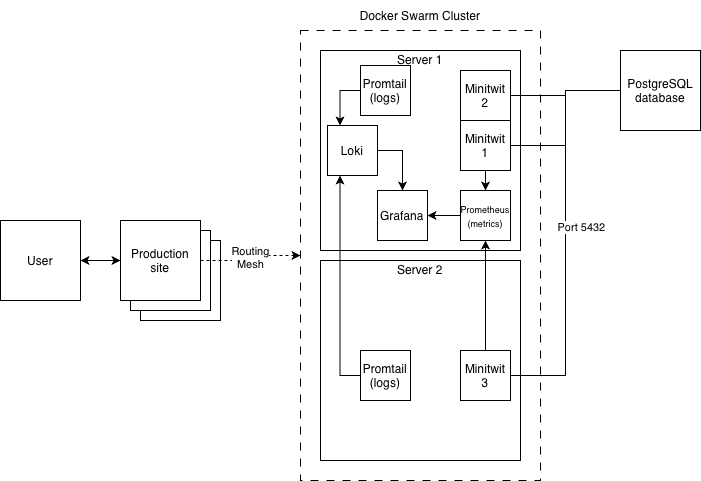
\includegraphics[width=1.2\textwidth]{img/Minitwit.png}}
    \caption{Architecture of the MiniTwit System}
    \label{fig:minitwit_arch}
\end{figure}

\subsection{Design \& Architecture}
\subsubsection{Application}
The minitwit application is a webapp twitter-like clone with simple functionality where users of the application can post tweets and follow each other.The application is written in Python with Jinja templates. The application has an API that contains the same functionality as the webapp. 
\subsubsection{Infrastructre}
\noindent\textbf{Infrastructure}\newline
Our system runs on three droplets hosted on DigitalOcean. Two swarm nodes form our swarm cluster. Minitwit-server 1 acts as a manager-worker and Minitwit-server 2 solely a worker. The last droplet is dedicated to hosting the sytem's Postgress database.\\

\noindent Besides managing container orchestration Mnitwit-server 1 is hosting 2 application replicas, a Promtail, Loki and Grafana replica. Minitwit-server 2 is hosting 1 application replica and a Promtail replica. Niginx is used as a reversed-proxy listening for incoming requests at port:80/443. Nginx forwards the given request and then the routing mesh of docker swarm forwards the request to an available replica. The routing mesh of the swarm ensures that each node in the cluster can handle any request regardless of which node is hosting the appropriate container. 
\subsubsection{Monitoring}
Our system monitors the web application using Prometheus, Loki, Promtail and Grafana. Docker has been used for containerization of the sytem's services.\newline 

\subsection{Dependencies}
\begin{figure}[h]
    \makebox[\textwidth][c]{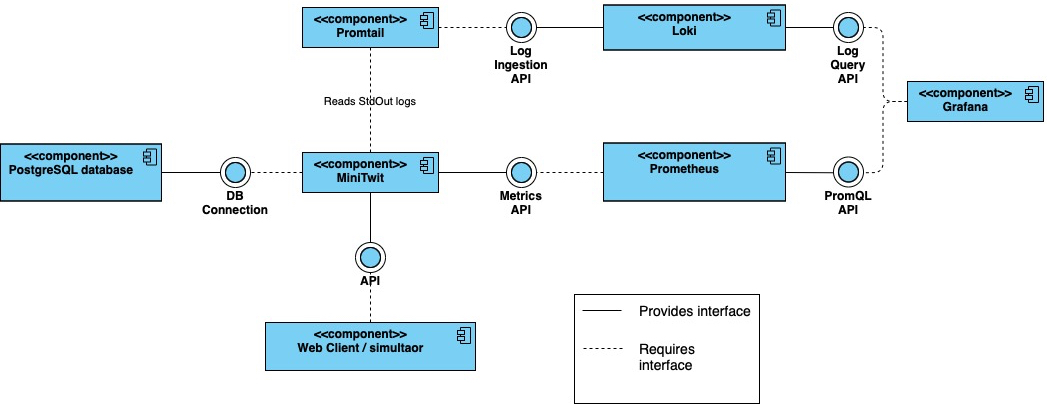
\includegraphics[width=1.4\textwidth]{img/Component_diagram-3.jpg}}
    \caption{Component diagram of the MiniTwit system, showing provided interfaces and dependencies between the core application, database and monitoring services}
    \label{fig:minitwit_arch}
\end{figure}
\subsubsection{Infrastructure}
\begin{itemize}
    \item \textbf{DigitalOcean Droplets}: Provides the hardware (CPU, Memory, Storage) to run a Linux OS on, hosting our services.
    \item \textbf{Docker}: Allows us to containerize our services.
    \item \textbf{Docker Swarm}: A part of Docker, allowing us to handle horizontal scaling and manage container health, update strategies and general management.
    \item \textbf{PostgreSQL}: A relational database management system, allowing us to write and read messages, log-in data and user-data concurrently.
\end{itemize}

\subsubsection{Application}
\begin{itemize} 
	\item \textbf{fastapi}: The asynchronous web framework handling routing, requests, and endpoints. 
	\item \textbf{uvicorn}: The web server deployment dependency used to run the FastAPI application.
	\item \textbf{Jinja2}: The template engine used for server-side rendering of user timelines and layouts. 
	\item \textbf{sqlmodel} / \textbf{SQLAlchemy}: The ORM used to abstract database interactions into Python code. 
	\item \textbf{psycopg2-binary}: The PostgreSQL  adapter required to handle high-concurrency network communication with our database container. 
	\item \textbf{Werkzeug} / \textbf{itsdangerous} : Cryptographic utility relied upon for password hashing (\textbf{generate\_password\_hash}) and session tokens. 
\end{itemize}

\subsubsection{Monitoring}
\begin{itemize}
    \item \textbf{Prometheus}: A systems monitoring toolkit used to scrape and monitor time-series metrics.
    \item \textbf{Loki:} A log scraper that aggregates application text logs.
    \item \textbf{Promtail}: A service attached to all containers, which streams container stdout logs to Loki.
    \item \textbf{Grafana}: A data visualization and analytics web application, allowing us to query and monitor the output of the above and organize it in dashboards.
\end{itemize}

\subsubsection{Pipeline}
\begin{itemize}
    \item \textbf{GitHub Actions}: Our CI/CD platform that automates our deployment, testing and building.
    \item \textbf{Docker Buildx and QEMU}: Compilation tools allowing us to create Docker Images that are agnostic to the OS they're being run on.
    \item \textbf{Black}: A code formatting tool allowing us to ensure an identical code style.
    \item \textbf{Hadolint}: An analysis tool that scans docker images for known vulnerabilities.
    \item \textbf{ShellCheck}: An analysis tool that scans shell files for bugs, syntax errors and vulnerabilities.
\end{itemize}

\subsection{Current System State}
\textit{Describe the current state of your systems, for example using results of static analysis and quality assessments.}
% for example using results of static analysis and quality assessments.